\documentclass[11pt]{article}
\usepackage{amsmath,amssymb,amsthm}
\usepackage{graphicx}
\usepackage{hyperref}
\usepackage{lmodern}
\usepackage{enumitem}

% Bibliography
\usepackage{natbib}
\bibliographystyle{aer}

% Page settings
\usepackage{setspace}
\onehalfspacing
\usepackage[margin=1in]{geometry}

% Variables
%%%%%%%%%%%%%%%%%%
% Definitions	%
%%%%%%%%%%%%%%%%%%

% Cost functions
\newcommand\cscore{c_{y}}
\newcommand\ctime{c_{t}}

% Distribution
\newcommand\fos[1]{ F^{\prime}_{X_{#1:n}}}

% Equilibrium
\newcommand\bidscore{y^*}
\newcommand\bidtime{t^*}
\newcommand\marginaltype{\bar x}
\newcommand\invertb{b^{-1}}

% Parameters
\newcommand\lowercost{\underline{c}}
\newcommand\uppercost{\bar{c}}
\newcommand\deadline{d}
\newcommand\target{\bar y}

\newcommand\entrylimit{\bar \theta}

% Expectations
\newcommand{\Expect}{\mathop{\bf E{}}}

% Sets
\newcommand\realsp{\mathbb{R}^{+}}

% Theorems
\newtheorem{proposition}{Proposition}



% Title page
\title{%
Races versus tournaments -- the model}
\date{%
Current version: \today}
\author{%
Andrea Blasco\thanks{%
  Email: \texttt{ablasco@fas.harvard.edu}}
}

\begin{document}
\maketitle
\begin{abstract}
We want compare races and tournaments in one single common framework. Here, we are going to build a new framework then estimate the \emph{primitives} of the model, and simulate data to show under what conditions one mechanism dominates the other.
\end{abstract}

\section{The model}
\begin{enumerate}[label=>>]

\item Consider $n+1$ agents competing in a contest over $k$ prizes of value $V_1 > V_2 > ... > V_k$.

\item To be eligible for the $j$'th prize, an agent has to complete a task within a deadline $d$ and produce an output that is ranked $j$'th in the competition. The output is evaluated and ranked by the sponsor of the contest along two dimensions. 

\item Let $y_i\in\realsp$ denote the first dimension indicative of an agent $i$'s output quality. And let $t_i\in\realsp$ denote the second that is indicative of the time to complete the task. 

\item In a tournament, agents who completed the task in time $t_i\leq d$ are then ranked by their output quality. Let $y_{r:n+1}$ denote the $r$'th smallest value of the $y_i$'s ($y_{1:n+1}$ being the smallest, $y_{2:n+1}$ being the second smallest, and so on). Then the agent having achieved the highest quality $y_{n+1:n+1}$ is ranked first and gets the first prize, the agent having achieved the second highest quality $y_{n:n+1}$ is awarded the second prize, and so on.

\item In a race, agents are required to meet a minimum quality which we denote $q$. Agents who complete the task in time and meet this requirement are then ranked by their time to complete the task. As before, let $t_{r:n+1}$ denote the $r$'th smallest time to achieve the minimum quality requirement of the $t_i$'s.  Then the agent being the first to achieve the required quality $t_{1:n+1}$ is ranked first and gets the first prize, the agent being the second $t_{2:n+1}$ is awarded the second prize, and so on. 


\item FOOTNOTE: Since time and quality are continuous variables we do not need to consider what happens when there are ties.
\item FOOTNOTE The case in which agents are ranked by a (linear) combination of time and quality can been studied as the traditional one-dimensional case. 

\item Output requires effort and each agent incurs a cost from effort that is increasing in the output's quality and decreasing in the output's timing (achieving output of higher quality requires time and time is costly). This cost is represented by the multiplicative cost function (e.g., Cobb-Douglas) 
\begin{equation}
  C(y, t) = \gamma(y) \delta(t) 
\end{equation}
with $\gamma(0)=0$, $\gamma^\prime>0$, $\delta(d)=\delta_0>0$, and $\delta^\prime<0$.

\item The individual ability of a player $x_i\in\realsp$, which we will also call her ``type,'' will shift these costs down (or up) by a factor $1/x_i$. 

\item Ability is privately observed by the agent before making any decision. And it is common knowledge that types are iid with common distribution $F_X$ on the support $[\lowercost, \uppercost]$ with $\lowercost>0$ and $F_X$ everywhere differentiable.

\item Each agent face the same problem
\begin{equation}
  \begin{array}{ll}
    \mbox{maximize} & \sum_{j=1}^k \Pr(\text{ranked $j$'th}) V_j  - C(y_i, t_i) / x_i.
  \end{array}
\end{equation}

\item The sponsor of the contest chooses the rules of the competition including prize structure $\{V_j\}_{j=1}^k$, deadline $d$, target quality $q$, and competition format (race or tournament). The sponsor maximizes an objective function that is the sum of total quality $Y=\sum_{i=1}^{n+1} Y_i$, time spent $T=\sum_{i=1}^{n+1} T_i$ and prizes paid $V=\sum_{j=1}^k p_{j} V_j$ (with $p_j=1$ if the prize is awarded and $p_j=0$ otherwise). Hence, the problem faced  by the sponsor is
\begin{equation}
  \begin{array}{ll}
    \mbox{maximize} & \Expect{Y}  - c_t \Expect{T} - \Expect{V}
  \end{array}
\end{equation}
with the intensity of preferences towards time weighted by $c_t\geq 0$. 
\end{enumerate}

\subsection{Tournament}
\begin{enumerate}[label=>>]

\item Let consider the case of $2$ prizes for simplicity.

\item  We characterize the equilibrium strategy of a player in a tournament which we denote by $t^*$ and $y^*$.\footnote{The strategy is a mapping $b_i:[\lowercost, \uppercost]\rightarrow \mathbb{R}^+ \times \mathbb{R}^+$ that maps types to two real numbers for quality and time. We focus on symmetric equilibria. In a symmetric equilibrium, agents are using the same strategy and the strategy is an equilibrium (because information is imperfect we use the Bayesian Nash Equilibrium notion).} 


\item It is readily verifiable that $t_i^*= \deadline$ is a weakly dominant strategy  for every $x_i$ (any $t_i < \deadline$ is strictly dominated by $t_i=\deadline$ and any $t_i\geq \deadline$ leads to zero utility).


\item Since there is imperfect information each agent will view all $y_j$ with $j\neq i$ as random variables. Let $F_{Y_{j:n}}$ denote the distribution of the $j$th smallest value of the ($n$ less the agent) $Y_j$'s 

\item The problem faced by each agent $i$ is

\begin{equation}
  \begin{array}{ll}
    \mbox{maximize} & \Pr(y > Y_{n:n}) V_1 + \Pr(Y_{n:n} > y > Y_{n-1:n}) (y)  V_2 - C(y, t) / x  
  \end{array}
\end{equation}

Using the distribution we have:
\begin{equation}
  \begin{array}{ll}
    \mbox{maximize} & F_{Y_{n:n}} (y) V_1 + [1 - F_{Y_{n:n}} (y)] F_{Y_{n-1:n-1}} (y)  V_2 - C(y, t) / x 
  \end{array}
\end{equation}

    


\[
  \Pr(y \geq Y_{n:n}) V_1 + \sum_{r=1}^{k-1} \Pr(Y_{n+1-r:n} > y \geq Y_{n-r:n}) V_{r+1};
\]
and it is zero otherwise. That can be written
\[
  [1 - F_{Y_{n:n}}] V_1 +  \sum_{r=1}^{k-1} [1 - F_{Y_{1:n+1-r}}]  F_{Y_{n-r:n}} V_{r+1}.
\]


\item Suppose that $t_i=T$. Suppose further that the performance of other players is a monotone decreasing function of their type. So we have $Y_j = b(X_j)$ and $b^{-1}(Y_j) = X_j$.

\item This implies that we can use a simple change of variable to rewrite the payoff as a function of $F_X$. And we have:
\[
  [1-F_{X_{n:n}}(b^{-1}(y_i))]V_1 + \sum_{r=1}^{k-1} \Pr(Y_{n+1-r:n} > y_i \geq Y_{n-r:n}) V_{r+1};
\]
Using Bayesian rule and one of the properties of $iid$ order statistics to express conditional probability, we have
\[
  [1-F_{X_{n:n}}(b^{-1}(y_i))]V_1 + \sum_{r=1}^{k-1} (1 - F_{X_{1:n-r}}) F_{X_{n-r:n}} V_r
\]
\end{enumerate}

\section{In a tournament}
\begin{itemize}
\item Consider an agent $i$. 
\item Let $Y_1, ..., Y_{n}$ denote the scores of i's opponents.  
\item It is readily verified that $t^*_i = d$ is a dominant strategy (any $t_i<d$ yields higher costs without affecting the probability of winning). [if we assumed that $t_i\leq d$]
\item The agent faces the following problem
\[
    \begin{array}{ll}
        \mbox{maximize} & \Pr(y_i > Y_{n:n}) V - x_i C(y_i, d)
    \end{array}
\]
where $y_i \in R_{+}$ is the optimization variable.
\item In a symmetric equilibrium, we have $Y_{n:n} = b(X_{n:n})$ with $b^{-1}$ denoting the inverse of $b(\cdot)$. Hence, the problem can be written as
\[
    \begin{array}{ll}
        \mbox{maximize} & [1- F_{X_{n:n}}(b^{-1}(y_i))] V - x_i C(y_i, d)
    \end{array}
\]
\item The first order condition is
\[
   - F_{X_{n:n}}^\prime(b^{-1}(y_i))] \frac{1}{b^\prime(b^{-1}(y_i))}V = x_i C^\prime(y_i, d).
\]
At equilibrium, we have
\[
    - F_{X_{n:n}}^\prime(x_i) \frac{1}{b^\prime(x_i)}V  = x_i C^\prime(b(x_i), d) 
\]
by replacing $b^{-1}(y_i)= x_i$. By rearranging and integrating both sides, this leads to
\[
  -\int F_{X_{n:n}}^\prime(x_i) \frac{V}{x_i}d x_i =\int b^\prime(x_i)  C^\prime(b(x_i), d) d x_i
\]
\[
  -\int F_{X_{n:n}}^\prime(x_i) \frac{V}{x_i} d x_i =C(b(x_i), d) + constant
\]
\item To solve the differential equation we use $b(\uppercost) = 0$, 
\[
  - V \int_{\lowercost}^{\uppercost} F_{X_{n:n}}^\prime(z) \frac{1}{z} dz = C(0, d) + constant
\]
\item If the costfunction is separable, we have
\[
  b(x) = C^{-1}\left[ - \hat V \int_{\lowercost}^{\uppercost} F_{X_{n:n}}^\prime(z) \frac{1}{z} dz - \hat V \int_{\lowercost}^{x} F_{X_{n:n}}^\prime(z) \frac{1}{z} dz \right]
\]
where $\hat V =  V / \delta(d)$ (the reward per hours worked). 


\end{itemize}

\clearpage
\section{The model}\label{the-model}
Consider $k\geq 3$ agents competing over $n\geq 1$ prizes of value $V_1 > V_2> ...> V_n$. 

To enjoy the $i$'th prize, an agent has to perform a certain task (the same for everyone) and be ranked $i$'th in the competition. 

In a tournament, agents are ranked by their performance. So, the agent having achieved the highest performance gets the first prize, the one having achieved the second highest performance is awarded the second prize, and so on. In a race, agents are ranked by the time to perform. So, the first agent to achieve a given performance, which we denote $\bar Y$, gets the first prize, the second to achieve $\bar Y$ is awarded the second prize, and so on. In both cases, the taks must be performed within a given deadline $T$ otherwise agents are not eligible for prizes. 

Agents simultaneously choose a real number $y\geq 0$ that is representative of their performance and a real number $t\geq 0$ that is the time to perform the task. Each agent incurs a cost from performing the task that is increasing in the performance level and decreasing in the time to perform. This cost is represented by the multiplicative cost function (like the Cobb-Douglas) 
\begin{equation}
  C(x, t) = \gamma(x) \delta(t) 
\end{equation}

with $\gamma(0)=0$, $\gamma^\prime>0$, $\delta(T)=1$, $\delta^\prime<0$.
%(e.g., $\delta(t)= e^{-t}$, $\delta(t)=T-t$). 

Agents are rational and make decisions to maximize an additive utility function. Each agent knows privately the weight attached to the cost function in her utility function. Let $X_1, ..., X_k$ denote these weights. It is common knowledge that $X_1,..., X_k$ are iid with common distribution $F$ on the support $[a, b]$ with $F$ being everywhere differentiable. Thus, the utility for an agent $k$ is:
\begin{equation}
  U_k = \sum_{i=1}^n P(\text{ranked $i$'th}) V_i - x_k C(y_k, t_k).
\end{equation}
Since there is private information on $X_i$, agents' choices are viewed as random variables by the other agents. Let $Y_1, ..., Y_k$ denote iid random variables distributed according to $F_Y$. Let $Y_{i:k-1}$ denote the $i$'th smallest of the $Y_i$. 
In a tournament, the probability of being ranked $i$'th can be expressed as the probability of the realized $y_k$ being higher than $i-1$'th order statistic and the $d$
Thus the utility can be written
\begin{equation}
  ... 
\end{equation}


\section{Equilibrium}
\subsection{The case of tournaments}

Consider the case of a competition with two prizes ($n=2$) and normalize the value of prizes to $V_1=\alpha$ and $V_2=1-\alpha$ so that the fraction $\alpha\leq 1/2$ denotes the fraction of the prize pool that goes to the winner (if $\alpha=1$ the winner gets all). 

The equilibrium of a tournament competition is described in the next proposition.

\begin{proposition}
Consider a tournament with $k\geq3$ agents, $n=2$ prizes, and $\alpha\leq 1/2$. Let $t^\star$ and $y^\star$ denote the equilibrium values.  It is a (weakly) dominant strategy to choose the time to submit $t^\star=T$. And, in a symmetric equilibrium, agents choose a score $y^\star=b(x)$ where 
\begin{equation}
  b(x) = [A(x) (1-\alpha) + B(x)\alpha]. 
\end{equation} 
where 
\begin{equation}
  A(c) = (k-1) \int_c^1 \frac{1}{a} [1-F(a)]^{k-2} F^\prime(a) da, 
\end{equation}
\begin{equation}
  B(c) = (k-1) \int_c^1 \frac{1}{a} [1-F(a)]^{k-3} [(k-1)F(a) - 1] F^\prime(a) da. 
\end{equation}
\end{proposition}

\begin{proof}
Let denote the $i$'th smallest value of the rivals $X_i$'s by $X_{i:k-1}$ (with $X_{1:k-1}$ being the smallest, $X_{2:k-1}$ being the second smallest, etc.). Then the distribution of $X_{i:k-1}$ can be easily derived \citep{arnold2012relations} and we have
\begin{equation}
  F_{X_{i:k-1}} (x) = \sum_{j=i}^{k-1} \binom{k-1}{j} F(x)^j (1-F(x))^{k-1-j}.
\end{equation}
And the corresponding density is
\begin{equation}
  f_{X_{i:k-1}} (x) = \frac{k-1!}{(i-1)!(k-1-i)!} F(x)^{i-1} (1-F(x))^{k-1-i} f(x). 
\end{equation}

Let $b^{-1}$ denote the inverse of the equilibrium xxx function. Then 
\begin{equation}
  b^{-1}(Y_j) =X_j. 
\end{equation}
and 
\begin{equation}
  b^{-1}(Y_{j:k-1}) =X_{j:k-1}. 
\end{equation}
(equal in distribution)

Then we have
\begin{equation}
  P(b^{-1}(Y_i) \geq X_{k-1:k-1})  = 1 - F_{X_{k-1:k-1}}(b^{-1}(Y_i)) .
\end{equation}

 we have that the probability of a competitor with a bid $x$ winning the first prize is equal to the probability of $b^{-1}(x)$ being the first order statistic of $k-1$ iid random bids.  

Hence, the problem faced by the agent is
\begin{equation}
\begin{split}
  \max  U = & F^\prime_{(1:k-1)}(b^{-1}{x}) (1-\alpha) + \\ 
        & + (1-F^\prime_{(1:k-1)}(b^{-1}{x})) F^\prime_{(1:k-2)}(b^{-1}{x}) \alpha + \\ 
        & - \gamma(x)\delta(T) \theta
\end{split}
\end{equation}
Let us call $F^\prime_{(1:k-1)} = g_{k-1}(x)$. Rearranging
\begin{equation}
\begin{split}
  \max  U = & g_{k-1}(b^{-1}{x}) (1-\alpha) + g_{k-2}(b^{-1}{x}) \alpha \\ 
        & - g_{k-1}(b^{-1}{x}) g_{k-2}(b^{-1}{x}) \alpha + \\ 
        & - \gamma(x)\delta(T) \theta
\end{split}
\end{equation}
First order condition: 
\begin{equation}
\begin{split}
  \max  U = & \frac{db^{-1}}{dx} [ g^\prime_{k-1}(b^{-1}{x}) (1-\alpha) +  g^\prime_{k-2}(b^{-1}{x}) \alpha + \\ 
  & - g^\prime_{k-1}(b^{-1}{x}) g_{k-2}(b^{-1}{x}) \alpha - g_{k-1}(b^{-1}{x})  g^\prime_{k-2}(b^{-1}{x}) \alpha ]+ \\ 
        & = \gamma^\prime(x)\delta(T) \theta
\end{split}
\end{equation}
In equilibrium $b^{-1}x = \theta$ and $d b^{-1}/ dx = 1/b^\prime(\theta)$
\begin{equation}
\begin{split}
  \max  U = & g^\prime_{k-1}(\theta) (1-\alpha) +  g^\prime_{k-2}(\theta) \alpha + \\ 
  & - g^\prime_{k-1}(\theta) g_{k-2}(\theta) \alpha - g_{k-1}(\theta)  g^\prime_{k-2}(\theta) \alpha  \\ 
        & = b^\prime(\theta) \gamma^\prime(b(\theta))\delta(T) \theta
\end{split}
\end{equation}
\end{proof}
 
\textit{Example uniform}

Consider $k=3$ and $F$ is uniform on $[m, 1]$ so that the CDF is $F(x)=(x-m) / (1-m)$.  Then, 
\begin{equation}
  A(c) = \frac{1-x}{(m-1)^2 x},
\end{equation}
\begin{equation}
  B(c) = -\frac{(1 + m - 2 x) (x-1)}{(m-1)^3 x}.
\end{equation}

\textit{1.2 Example lognormal}

\textit{1.2 Example Kumaraswamy}

Consider $F$ is Kumaraswamy on $(0,1)$ with shape parameters $s_1$ and $s_2$ and CDF equal to $1-(1-x^{s_1})^{s_2}$. When $s_1=s_2=1$ we have a uniform distribution.


\subsection{Expected utility}

Let $x_{(n)}$ denote the n-th order statistic of $k$ types. 
Then the expected payoff in equilibrium in both the race and the tournament but the costs are different. So the expected utility is
\begin{equation}
\Pr(\theta\leq\theta_{1:k-1}) (1-\alpha) + \Pr(\theta_{1:k-1}>\theta\leq\theta_{2:k-1}) \alpha - C(b_{to}(\theta), T, \theta).
\end{equation}
and 
\begin{equation}
\Pr(\theta\leq\theta_{1:k-1}) (1-\alpha) + \Pr(\theta_{1:k-1}>\theta\leq\theta_{2:k-1}) \alpha - C(Q, b_{ra}(\theta), \theta).
\end{equation}


\section{Empirical analysis}

Consider $n$ observations from the same type of competition. Our dataset is $(y_i, x_i), ..., (y_n, x_n)$ where $y_i$ is a vector of time $t_i$ and scores $s_i$. 

For a tournament with $k$ competitors, our model gives the equilibrium relationship
\begin{equation}
  t_i = T \text{ and } s_i = b(\theta_i, F, \alpha)
\end{equation}
Suppose we know the distribution $F$ up to some parameter $\beta$, then we have
\begin{equation}
  s_i = b(\theta_i, \beta, \alpha). 
\end{equation}
Note that the score is linear in $\alpha$ but nonlinear in $\beta$. 


Suppose the observed relationship is nondeterministic, and assume that our model is correct on average. That is, the conditional mean of scores is 
\begin{equation}
  E[s_i \mid x_i, \beta] = b(\theta_i, \beta, \alpha)
\end{equation}
For example, we assume
\begin{equation}
  s_i = b(\theta_i, \beta, \alpha) + \epsilon_i
\end{equation}
and errors are assumed to be normally distributed with mean zero. 

The parameters are estimated by min residual summ of squares (RSS) with respect to $\beta$ and $\alpha$. 
\begin{equation}
  RSS(\beta, \alpha) = \sum_{i=1}^{n} (y_i - b(x_i))^2
\end{equation}




\textbf{Censoring}

\emph{Lots of zeros}. It could be that people participated but did not submit their solutions so that zeros are missing observations. However, this situation seems unlikely given that to win you need to submit solutions and get feedback. In reality, we believe that a zero submission is a competitor who dropped the competition.

\emph{Drop outs}. Reasons are they see their rivals and decide to quit. This is consistent with theory. High number of drop outs suggests our model fits better with a fixed cost. 

\appendix
\section{Order statistics}
Following \cite{arnold2012relations}, we let $X_1, ..., X_n$ denote $n$ jointly distributed random variables. We denote the i'th smallest of the $X_i$'s by $X_{i:n}$ ($X_{1:n}$ being the smallest, $X_{2:n}$ being the second smallest, etc.). 


If $X_1, ..., X_n$ are iid with common distribution $F$, the distribution of an individual order statistic is
\begin{equation} \label{eq: distribution}
  F_{X_{i:n}} (x) = 
  P(X_{i:n} \leq x) = \sum_{j=i}^{n} \binom{n}{j} F(x)^j (1-F(x))^{n-j}. 
\end{equation}
Another representation is possible. Consider $U_1,...,U_n$ denote iid variables with uniform distribution on the unit interval.  Define the inverse $F^{-1}(x)$. It is readily verified that 
\begin{equation}
  F^{-1}(U_i) = X_i
\end{equation}
and 
\begin{equation}
  F^{-1}(U_{i:n}) = X_{i:n}.
\end{equation}
Now the distribution \eqref{eq: distribution} (replace $F(u)$ with $u$) is absolutely continuous  with corresponding density:
\begin{equation}
  f_{U_{i:n}} (u) = \frac{n!}{(i-1)!(n-i)!} u^{i-1} (1-u)^{n-i}.
\end{equation}
The distribution can then be written:
\begin{equation}
  F_{U_{i:n}} (u) = \int_{0}^u \frac{n!}{(i-1)!(n-i)!} t^{i-1} (1-t)^{n-i} dt
\end{equation}
This yields the general expression
\begin{equation}
  F_{X_{i:n}} (x) = \int_{0}^F(x) \frac{n!}{(i-1)!(n-i)!} t^{i-1} (1-t)^{n-i} dt
\end{equation}

If $F(x)$ is everywhere differentiable, then the density is
\begin{equation}
  f_{X_{i:n}} (x) = \frac{n!}{(i-1)!(n-i)!} F(x)^{i-1} (1-F(x))^{n-i} f(x). 
\end{equation}

Another important result is the probability of being in between two values
\begin{equation}
  P (X_{j:n} > x > X_{i:n})
\end{equation}
with $i<j$. We can use bayes and we have
\begin{equation}
  P (X_{i:n} > x > X_{j:n}) = P ( x > X_{j:n} | X_{i:n} > x ) P (X_{i:n} > x)
\end{equation}
Important result: for $i< j$ the conditional distribution of $X_{j:n}$ given $X_{i:n}=x$ is the same as the unconditional distribution of $Y_{j-i: n-i}$

\begin{figure}
\centering
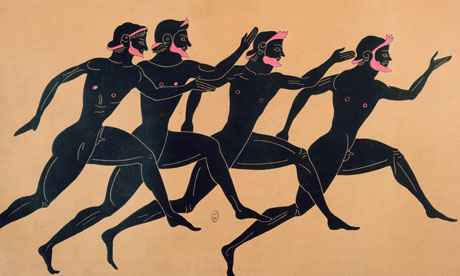
\includegraphics[width=0.5\textwidth]{img/racer.jpg}\\
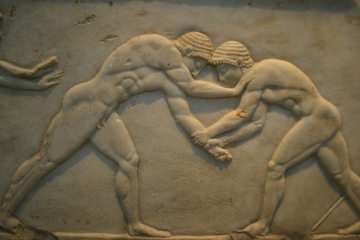
\includegraphics[width=0.5\textwidth]{img/wrestler.jpg}
\caption{Greek racers and wrestlers}
\end{figure}


\tableofcontents

% Bibliography  ls

\newpage
\singlespacing
\bibliography{/Users/andrea/Papers/library}

\end{document}
